%%% Copyright (C) 2020 David Beauchemin
%%%
%%% Ce fichier et tous les fichiers .tex ou .Rnw dont la racine est
%%% mentionnée dans les commandes \include et \input ci-dessous font
%%% partie du projet «Maman, j'ai (encore) perdu les résultats de mon
%%% rapport! - Webinaire de la Formation continue FSG»
%%% https://gitlab.com/vigou3/webinaire-recherche-reproductible
%%%
%%% Cette création est mise à disposition selon le contrat
%%% Attribution-Partage dans les mêmes conditions 4.0
%%% International de Creative Commons.
%%% https://creativecommons.org/licenses/by-sa/4.0/

\documentclass[aspectratio=169,10pt,xcolor=x11names,english,french]{beamer}
\usepackage{babel}
\usepackage[autolanguage]{numprint}
\usepackage{amsmath}
\usepackage{currfile}                  % nom fichier de script
\usepackage{changepage}                % page licence
\usepackage{tabularx}                  % page licence
\usepackage{relsize}                   % \smaller et al.
\usepackage{awesomebox}                % boites signalétiques
\usepackage{fancyvrb}                  % texte verbatim
\usepackage{framed}                    % env. leftbar
\usepackage{pict2e}                    % cycle travail Git
\usepackage[overlay,absolute]{textpos} % couvertures
\usepackage{metalogo}       
\usepackage{textpos}           % logo \XeLaTeX

%% =============================
%%  Informations de publication
%% =============================
\title{Reproductibilité en apprentissage automatique}
\author{David Beauchemin}
\date{30 octobre 2020}
\newcommand{\reposurl}{...}

%% =======================
%%  Apparence du document
%% =======================

%% Thème Beamer général
\usetheme[titleformat=allcaps, numbering=none, block=transparent]{metropolis}

%% Modifications aux couleurs: fond blanc, titres en texte noir sur
%% fond blanc
\setbeamercolor{normal text}{bg=white}
\setbeamercolor{frametitle}{fg=normal text.fg, bg=}

%% Déplacer les titres vers le bas sous la décoration du gabarit CFDD
\makeatletter
\setlength{\metropolis@frametitle@padding}{4.9ex}
\renewcommand{\metropolis@frametitlestrut@start}{
	\rule{0pt}{6ex +%
		\totalheightof{%
			\ifcsdef{metropolis@frametitleformat}{\metropolis@frametitleformat X}{X}%
		}%
	}
}
\renewcommand{\metropolis@frametitlestrut@end}{}
\makeatother

%% Format de la page de titre de section; redéfinition pour insérer
%% la décoration du CFDD, aligner le titre à gauche et désactiver
%% l'hyperlien (https://tex.stackexchange.com/a/183357)
\makeatletter
\setbeamertemplate{section page}{%
	\begin{textblock*}{92.5mm}[1,1](160mm,90mm)
		
\includegraphics[height=\paperheight,keepaspectratio]{img/Élément2_PPT}
	\end{textblock*}
	\begin{minipage}{22em}
		\raggedright
		\usebeamerfont{section title}
		\let\hyperlink\@secondoftwo\textcolor[rgb]{0,0.29,0.37}{\insertsectionhead}\par
	\end{minipage}
	\par
	\vspace{\baselineskip}
}
\makeatother

%% Polices de caractères
\newfontfamily\Overpass{Overpass}
\setsansfont{Overpass}        % police principale
\newfontfamily\OverpassSemiBold{Overpass}
[
BoldFont = *-SemiBold
]
\newfontfamily\OverpassExtraLightBold{Overpass}
[
UprightFont = *-ExtraLight,
BoldFont = *-Light
]
\newfontfamily\OverpassLight{Overpass}
[
UprightFont = *-Light,
BoldFont = *-Regular
]

%% Couleurs additionnelles
\definecolor{comments}{rgb}{0.7,0,0}  % rouge foncé
\definecolor{link}{rgb}{0,0.4,0.6}    % liens internes
\definecolor{url}{rgb}{0.6,0,0}       % liens externes
\definecolor{codebg}{named}{LightYellow1} % fond code R
\definecolor{rouge}{rgb}{0.85,0,0.07} % bandeau rouge UL
\definecolor{or}{rgb}{1,0.8,0}        % bandeau or UL
\colorlet{alert}{mLightBrown} % alias pour couleur Metropolis
\colorlet{dark}{mDarkTeal}    % alias pour couleur Metropolis
\colorlet{code}{mLightGreen}  % alias pour couleur Metropolis
\colorlet{shadecolor}{codebg}

%% Hyperliens
\hypersetup{%
	pdfauthor = {Vincent Goulet},
	pdftitle = {Introduction à la science des données},
	colorlinks = {true},
	linktocpage = {true},
	allcolors = {link},
	urlcolor = {url},
	pdfpagemode = {UseOutlines},
	pdfstartview = {Fit},
	bookmarksopen = {true},
	bookmarksnumbered = {true},
	bookmarksdepth = {subsection}}

%% Paramétrage de babel pour les guillemets
\frenchbsetup{og=«, fg=»}

%% =========================
%%  Nouveaux environnements
%% =========================

%% Environnement pour le code informatique; hybride
%% des environnements snugshade* et leftbar de framed.
\makeatletter
\newenvironment{Scode}{%
	\def\FrameCommand##1{\hskip\@totalleftmargin
		\vrule width 3pt\colorbox{codebg}{\hspace{5pt}##1}%
		% There is no \@totalrightmargin, so:
		\hskip-\linewidth \hskip-\@totalleftmargin \hskip\columnwidth}%
	\MakeFramed {\advance\hsize-\width
		\@totalleftmargin\z@ \linewidth\hsize
		\advance\labelsep\fboxsep
		\@setminipage}%
}{\par\unskip\@minipagefalse\endMakeFramed}
\makeatother

%% Environnement pour le contenu d'un fichier; alias de snugshade*.
\newenvironment{Sfile}{\begin{snugshade*}}{\end{snugshade*}}

%% =====================
%%  Nouvelles commandes
%% =====================

%% Lien externe
\newcommand{\link}[2]{\href{#1}{#2~{\smaller\faExternalLink*}}}

%% Renvoi vers GitLab sur la page de copyright
\newcommand{\viewsource}[1]{%
	\href{#1}{\faGitlab\ Voir sur GitLab}}

%% Simili commande \HUGE
\newcommand{\HUGE}{\fontsize{36}{36}\selectfont}

%% Raccourcis usuels vg
\newcommand{\code}[1]{\textcolor{code}{\texttt{#1}}}

%%% =======
%%%  Varia
%%% =======

%% Longueurs pour la composition des pages couvertures avant et
%% arrière
\newlength{\banderougewidth} \newlength{\banderougeheight}
\newlength{\bandeorwidth}    \newlength{\bandeorheight}
\newlength{\imageheight}     \newlength{\imagewidth}
\newlength{\logoheight}

\begin{document}
	
	%% Style de l'entête et du pied de page: ajout des décorations du
	%% gabarit CFDD. Je ne sais pas pourquoi, mais si ces définitions se
	%% trouvent dans le préambule, le texte des diapos est déplacé vers le
	%% bas.
	\setbeamertemplate{headline}{%
		\ifnum\insertframenumber>1\relax%
		\begin{textblock*}{17mm}(0mm,0mm)
			
\includegraphics[width=\linewidth,keepaspectratio]{img/Élément4_PPT}
		\end{textblock*}
		\fi}
	\setbeamertemplate{footline}{%
		\ifnum\insertframenumber>1\relax%
		\begin{textblock*}{24.5mm}[1,1](160mm,90mm)
			
\includegraphics[width=\linewidth,keepaspectratio]{img/Élément3_PPT}
		\end{textblock*}
		\fi}
	
	%% frontmatter
	%%% Copyright (C) 2020 David Beauchemin
%%%
%%% Ce fichier et tous les fichiers .tex dont la racine est
%%% mentionnée dans les commandes \include et \input ci-dessous font
%%% partie du projet «Reproductibilité en apprentissage automatique
%%% - Webinaire de l'AAIARD»
%%% https://davebulaval.github.io/reproductibilite-en-apprentissage-automatique/
%%%
%%% Le format et le visuel est très fortement inspiré du matériel de
%%% Vincent Goulet https://gitlab.com/vigou3/webinaire-recherche-reproductible
%%%
%%% Cette création est mise à disposition selon le contrat
%%% Attribution-Partage dans les mêmes conditions 4.0
%%% International de Creative Commons.
%%% https://creativecommons.org/licenses/by-sa/4.0/

%% Normes de présentation visuelle 2018
%%
%% - grille de 8 unités de haut
%% - 1 mesure = 1/8 d'unité
%% - bande identitaire de 1 mesure placée au bas de la 7e unité
%% - logo haut de 4 mesures avec blancs de deux mesures en haut et
%%   en bas
%% - blanc équivalent à la largeur du blason à droite du logo
%% - bande or de la largeur du logo + blanc à droite
%%
%% Dimensions du logo UL
%%
%% hauteur: 129
%% largeur totale: 312
%% largeur blason: 102
%% valeur clé: (312 + 102)/129 = 3.209302
%%
%% Dimensions de l'image
%%
%% hauteur: 55 mesures - 1pt (filet) = 54.9191919 mesures
%% largeur: 160mm
%% ratio largeur/hauteur: 160/77.23

\begingroup
\TPGrid{16}{64}
\textblockorigin{0mm}{0mm}
\setlength{\parindent}{0mm}
\setlength{\imageheight}{54.9191919\TPVertModule}
\setlength{\logoheight}{4\TPVertModule}
\setlength{\bandeorwidth}{3.209302\logoheight}
\setlength{\banderougewidth}{\paperwidth}
\addtolength{\banderougewidth}{-\bandeorwidth}
\setlength{\bandeorheight}{\TPVertModule}
\setlength{\banderougeheight}{\TPVertModule}
\setlength{\textwidth}{\paperwidth}
\addtolength{\textwidth}{-2\TPHorizModule}

\def\titlefmt{%
  \bfseries\fontsize{24}{24}\selectfont%
  REPRODUCTIBILITÉ EN \\APPRENTISSAGE AUTOMATIQUE\par}
\def\webinaire{%
  \OverpassSemiBold\bfseries\fontsize{18}{18}\selectfont
  WEBINAIRE}
\def\datefmt{%
  \OverpassExtraLightBold\bfseries\fontsize{14}{14}\selectfont%
  15 DÉCEMBRE 2020}

%%%
%%% Page de titre
%%%
\begin{frame}[plain]
	%% bandeau identitaire
	\begin{textblock*}{\paperwidth}[0,1](0mm,56\TPVertModule)
		\textcolor{rouge}{\rule{\banderougewidth}{\banderougeheight}}%
		\textcolor{bleu}{\rule{\bandeorwidth}{\bandeorheight}}
	\end{textblock*}
	
	%% identifiant «webinaire»
	\begin{textblock*}{2\TPHorizModule}(0.7\TPHorizModule,5\TPVertModule)
		\textcolor[rgb]{0.13,0.13,0.13}{\webinaire}
	\end{textblock*}
	
	%% titre
	\begin{textblock*}{12\TPHorizModule}(0.7\TPHorizModule,17\TPVertModule)
		\textcolor[rgb]{0.13,0.13,0.13}{\titlefmt}
	\end{textblock*}
	
	%% date
	\begin{textblock*}{10\TPHorizModule}(0.7\TPHorizModule,41\TPVertModule)
		\textcolor[rgb]{0.13,0.13,0.13}{\datefmt}
	\end{textblock*}
\end{frame}
\endgroup

	
	\begin{frame}{Objectifs de la présentation}
		\begin{itemize}
			\item Sensibiliser sur les enjeux de la reproductibilité.
			\item Inciter l'intégration des solutions permettant une meilleure reproductibilité dans vos solutions d'affaires ou académiques.
			\item Améliorer votre productivité.
		\end{itemize}
	\end{frame}
	
	\begin{frame}
		\frametitle{Votre conférencier}
		
		\begin{minipage}{0.25\linewidth}
			
\includegraphics[width=\linewidth,keepaspectratio]{img/david}
		\end{minipage}
		\hfill
		\begin{minipage}{0.70\linewidth}
			\begin{itemize}
				\item Introduit à la recherche reproductible en 2016 (R Markdown et Git)
				\item Participation à REPROLANG de la conférence LREC \cite{garneau2020robust}
				\item Membre actif dans le développement d'une librairie facilitant la reproductibilité (\href{https://poutyne.org/}{Poutyne})
			\end{itemize}
		\end{minipage}
		
		\begin{minipage}{0.25\linewidth}
			\small
			\textbf{DAVID BEAUCHEMIN} \\
			Candidat au doctorat \\
			Département d'informatique et de génie logiciel
		\end{minipage}
	\end{frame}
	
	\section{Introduction}
	\begin{frame}{C'est quoi la reproductibilité ?}
		La reproductibilité est le principe qu'on ne peut tirer de conclusions que d'un événement bien décrit, qui est apparu plusieurs fois, provoqué par des \textbf{personnes différentes}.
		
		Toutefois, on utilise souvent ce terme pour spécifiquement désigner la \textbf{réplicabilité}. Soit la réplication (reproduction) des résultats d'un article dans des environnements pas (toujours) différents \cite{replicationvsreproductiblity, pineau2020improving}.
	\end{frame}
	
	\begin{frame}{En somme}
		\begin{itemize}
			\item<1-> Être capable de \textbf{répliquer} les résultats d'un article/ d'un projet,
			\item<2-> à partir du \textbf{même jeu de données} ou un jeu de données différent (mais proche),
			\item<3-> en utilisant la \textbf{procédure d'entrainement} de l'article ou en utilisant notre procédure d'entrainement et
			\item<4-> en utilisant le \textbf{code du projet}.
		\end{itemize}
	\end{frame}
	
	\begin{frame}{Pourquoi s'y intéressé?}
		\begin{itemize}
			\item<1-> $70$~\% des chercheurs en science on échoué dans leur tentative de reproduire un article d'un autre chercheur,
			\item<2-> ~$50$~\% n'ont pas réussit à reproduire leurs \textbf{propres} expérimentations \cite{baker500ScientistsLift2016}.
		\end{itemize}
		\uncover<3->{L'informatique ne fait pas exception à cela malgré la simplicité (théorique) de réplication des résultats. Selon une étude, sur 255 articles près de $40$~\% n'était pas réplicable \cite{raff2019step}.}
	\end{frame}
	
	\begin{frame}{Motivation}
		La reproductibilité facilite la réutilisation pour d'autres projets de recherche, améliorer votre productibilité \textbf{et} permet le transfert vers l'industrie (plus facilement). 
	\end{frame}
	
	\section{Les barrières à la réplicabilité}
	\begin{frame}
		\begin{itemize}
			\item<1-> Non-disponibilité du jeu de données ou \textbf{version} (pas clair) du jeu de données, 
			\item<2-> \textbf{mauvaise spécification ou sous-spécification} du modèle et de la \textbf{procédure d'entraînement},
			\item<3-> manque de \textbf{disponibilité du code} nécessaire pour exécuter les expériences, ou \textbf{erreurs} dans le code,
			\item<4-> \textbf{configurations} du modèle déficientes \cite{pineau2020improving}\footnote{Liste sélective}.
		\end{itemize}
	\end{frame}
	
	\begin{frame}
		\begin{figure}
			\centering
			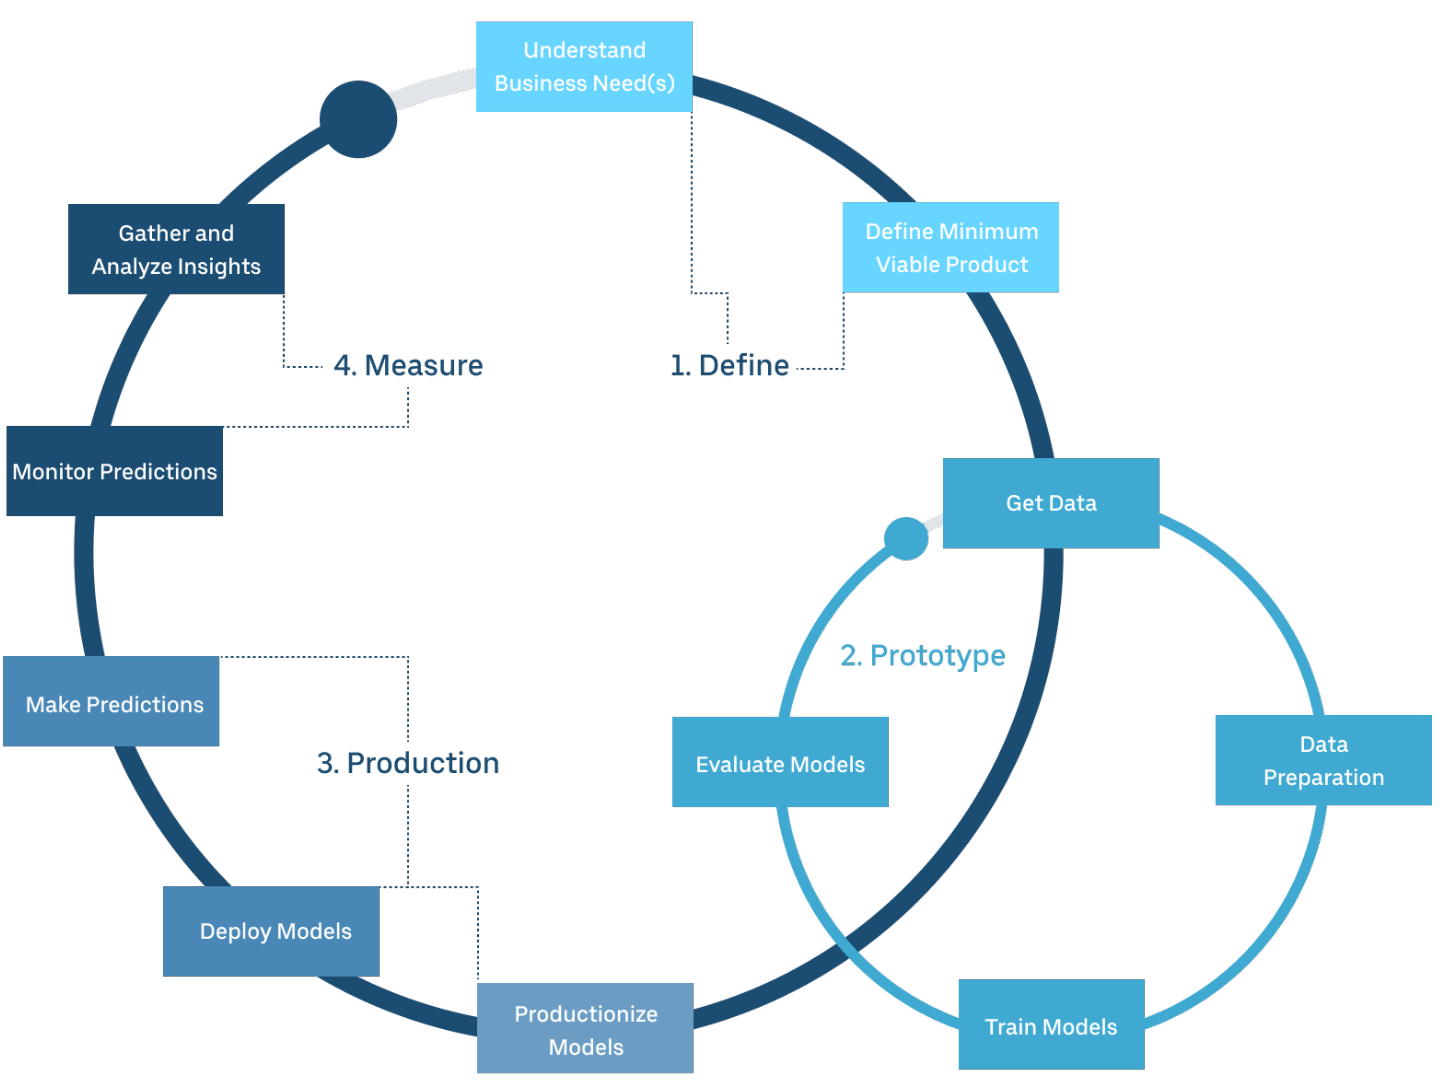
\includegraphics[scale=0.19]{img/cycle.png}
			\caption{\href{https://eng.uber.com/scaling-michelangelo/}{From Uber Engineering}}
		\end{figure}
	\end{frame}
	
	\begin{frame}
		\begin{figure}
			\centering
			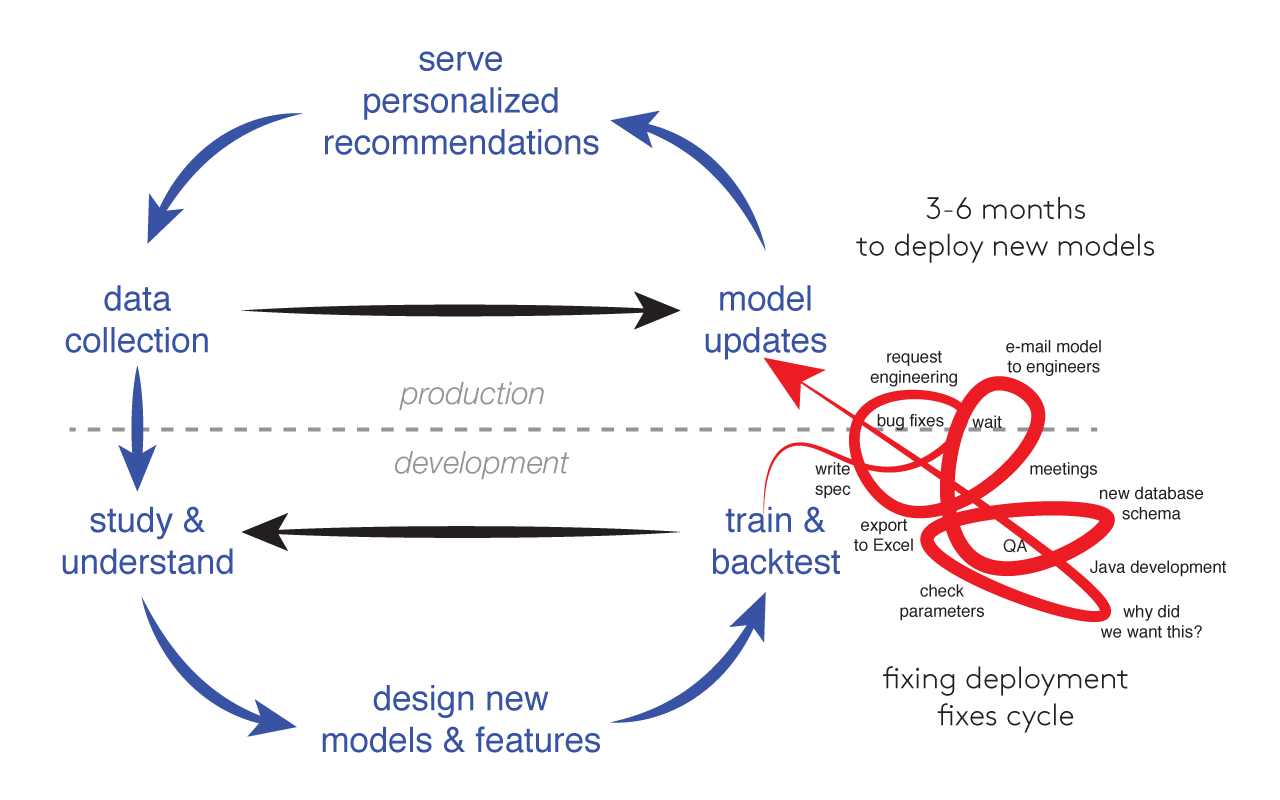
\includegraphics[scale=0.24]{img/cycle-white.png}
			\caption{\href{https://johann.schleier-smith.com/blog/2015/08/09/need-for-agile-machine-learning.html}{The need for Agile machine learning}}
		\end{figure}
	\end{frame}
	
	\section{OK, mais comment?}
	
	\begin{frame}
		\begin{figure}
			\centering
			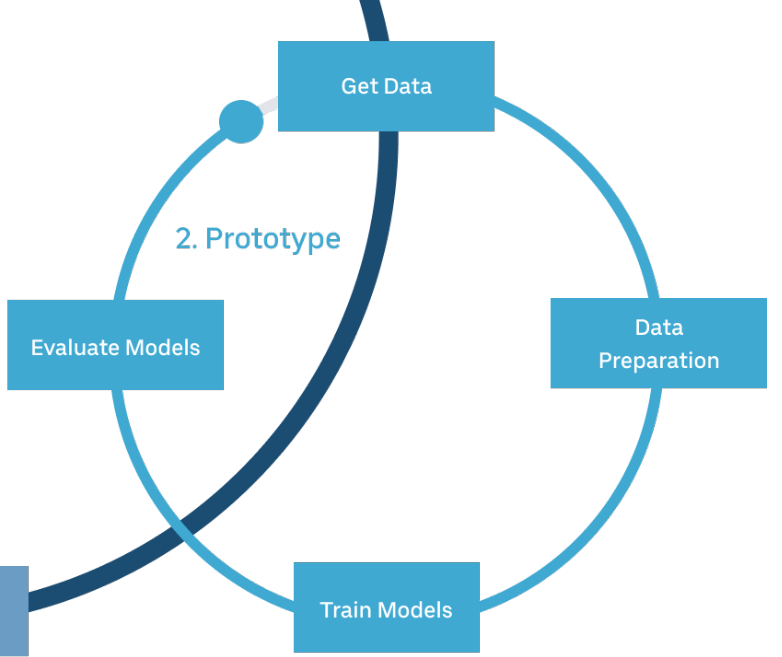
\includegraphics[scale=0.3]{img/cycle-2.png}
			\caption{\href{https://eng.uber.com/scaling-michelangelo/}{From Uber Engineering}}
		\end{figure}
	\end{frame}
	\subsection{Données}
	\begin{frame}{Version des données \& Étapes de pré procession}
		\begin{itemize}
			\item<1-> Avec qu'elle version des données doit-on travailler?
			\item<2-> Comment gérer \textbf{facilement} plusieurs versions des données?
			\item<3-> Comment définir \textbf{facilement} les étapes de pré procession des données?
		\end{itemize}
		\uncover<4->{Il nous faut des \textit{\textbf{data pipelines}}, des tuyaux que nous pouvons raccorder \textbf{facilement} à nos modèles pour l'entrainement et la mise en production, par exemple, Data Version Control (\href{https://dvc.org/}{DVC}).}
	\end{frame}
	
	\subsection{Codes}
	\begin{frame}{Version du code}
		\begin{itemize}
			\item<1-> Avec qu'elle version du code doit-on travailler?
			\item<2-> Comment savoir \textbf{rapidement} qu'elle est la différence d'implémentation entre deux versions du modèle?
			\item<3-> Comment gérer \textbf{facilement} les embranchements d'expérimentations?
		\end{itemize}
		\uncover<4->{Il nous faut un outil nous permettant de \textbf{visualiser} la différence entre des fichiers de code et nous permettant d'avoir \textbf{plusieurs} versions du code \textbf{\guillemotleft en même temps \guillemotright}, par exemple, \href{https://git-scm.com/}{Git}.}
	\end{frame}
	
	\subsection{Développement}
	\begin{frame}{Développement des modèles}
		\begin{itemize}
			\item<1-> Ne pas réinventer la roue.
			\item<2-> Simplifier l'écriture de code pour développer des modèles.
			\item<3-> Qui facilite l'entrainement (GPU, multi-GPU/CPU).
		\end{itemize}
		\uncover<4->{Il nous faut des outils nous permettant de \textbf{simplifier} le \textbf{développement} de nos modèles, par exemple, Poutyne \cite{poutyne}, PyTorch Lightning \cite{falcon2019pytorch}, Scikit-Learn \cite{sklearn_api}, Gensim \cite{rehurek_lrec} et Allen NLP \cite{Gardner2017AllenNLP}.}
	\end{frame}
	
	\begin{frame}{Entraînement, configuration et résultats}
		\begin{itemize}
			\item<1-> Avec qu'elle version du code, du modèle et des données avons-nous fait cet entrainement?
			\item<2-> Quels sont les résultats?
			\item<3-> Comment visualiser \textbf{rapidement} les résultats et les paramètres de configuration?
		\end{itemize}
		\uncover<4->{Il nous faut des outils nous permettant de \textit{\textbf{logger}} les \textbf{paramètres} d'entrainement et les \textbf{résultats}, par exemple, MLFlow \cite{Zaharia2018AcceleratingTM} et Sacred \cite{sacred}.}
	\end{frame}
	
	\begin{frame}{Rapport et analyse des résultats}
		\begin{itemize}
			\item<1-> Comment créer des tableaux de résultats \textbf{facilement} (pas à la \textit{mitaine})?
			\item<2-> Comment s'assurer \textbf{facilement} que les résultats sont à jours?
			\item<3-> Comment visualiser \textbf{rapidement} les résultats et les paramètres de configuration?
		\end{itemize}
		\uncover<4->{Il nous faut des outils nous permettant de \textbf{créer} des tableaux de résultats \textbf{à même les résultats}, soit de diminuer le plus possible le travail manuel, par exemple, \href{https://github.com/jsleb333/python2latex}{Python2LaTeX} et \href{https://fr.wikipedia.org/wiki/Markdown}{Markdown} .}
	\end{frame}
	
	\begin{frame}{Dockerisation}
		\begin{itemize}
			\item<1-> Comment s'assurer que nos modèles fonctionnent sur d'autres environnements?
			\item<2-> Comment faciliter la réutilisation de notre code?
		\end{itemize}
		\uncover<3->{\href{https://www.docker.com/}{Docker}!}
	\end{frame}
	
	%https://gitlab.com/vigou3/webinaire-recherche-reproductible
	
	
	\section{La suite}
	\begin{frame}
		Développer des processus rigoureux (par essai et erreur) et ne pas prendre tout ce qui a été discuté ici comme l'unique solution.
	\end{frame}
	
	\begin{frame}{Pour aller plus loin}
		\begin{itemize}
			\item \href{https://www.oreilly.com/library/view/clean-code-a/9780136083238/}{Clean code}
			\item \href{https://github.com/iterative/cml}{Continuous Machine Learning}
			\item Faire des tests!
			\item Writing Code for NLP Research \cite{gardner-etal-2018-writing}
		\end{itemize}
	\end{frame}
	
	\begin{frame}
		\frametitle{Période de questions}
		
		\centering
		\fontsize{100}{100}\selectfont
		\faQuestion
		
	\end{frame}
	
	\begin{frame}[t, allowframebreaks]
		\frametitle{References}
		\bibliographystyle{apalike}
		\bibliography{RAA}
	\end{frame}
	
	%%% Copyright (C) 2020 David Beauchemin
%%%
%%% Ce fichier et tous les fichiers .tex dont la racine est
%%% mentionnée dans les commandes \include et \input ci-dessous font
%%% partie du projet «Reproductibilité en apprentissage automatique
%%% - Webinaire de l'AAIARD»
%%% https://davebulaval.github.io/reproductibilite-en-apprentissage-automatique/
%%%
%%% Le format et le visuel est très fortement inspiré du matériel de
%%% Vincent Goulet https://gitlab.com/vigou3/webinaire-recherche-reproductible
%%%
%%% Cette création est mise à disposition selon le contrat
%%% Attribution-Partage dans les mêmes conditions 4.0
%%% International de Creative Commons.
%%% https://creativecommons.org/licenses/by-sa/4.0/

%% Normes de présentation visuelle 2018
%%
%% - grille de 8 unités de haut
%% - 1 mesure = 1/8 d'unité
%% - bande identitaire de 1 mesure placée au bas de la 7e unité
%% - logo haut de 4 mesures avec blancs de deux mesures en haut et
%%   en bas
%% - blanc équivalent à la largeur du blason à droite du logo
%% - bande or de la largeur du logo + blanc à droite
%%
%% Dimensions du logo UL
%%
%% hauteur: 129
%% largeur totale: 312
%% largeur blason: 102
%% valeur clé: (312 + 102)/129 = 3.209302
%%
%% Dimensions de l'image
%%
%% hauteur: 55 mesures - 1pt (filet) = 54.9191919 mesures
%% largeur: 160mm
%% ratio largeur/hauteur: 160/77.23

\begingroup
\TPGrid{16}{64}
\textblockorigin{0mm}{0mm}
\setlength{\parindent}{0mm}
\setlength{\imageheight}{54.9191919\TPVertModule}
\setlength{\logoheight}{4\TPVertModule}
\setlength{\bandeorwidth}{3.209302\logoheight}
\setlength{\banderougewidth}{\paperwidth}
\addtolength{\banderougewidth}{-\bandeorwidth}
\setlength{\bandeorheight}{\TPVertModule}
\setlength{\banderougeheight}{\TPVertModule}
\setlength{\textwidth}{\paperwidth}
\addtolength{\textwidth}{-2\TPHorizModule}

\def\titlefmt{%
	\bfseries\fontsize{24}{24}\selectfont%
	MERCI DE VOTRE \\ ÉCOUTE!\par}
\def\webinaire{%
	\OverpassSemiBold\bfseries\fontsize{18}{18}\selectfont
	WEBINAIRE}

%%%
%%% Page de titre
%%%
\begin{frame}[plain]
	%% bandeau identitaire
	\begin{textblock*}{\paperwidth}[0,1](0mm,56\TPVertModule)
		\textcolor{rouge}{\rule{\banderougewidth}{\banderougeheight}}% % bande rouge
		\textcolor{bleu}{\rule{\bandeorwidth}{\bandeorheight}}           % bande or
	\end{textblock*}
	
	%% identifiant «webinaire»
	\begin{textblock*}{10\TPHorizModule}(0.7\TPHorizModule,5\TPVertModule)
		\textcolor[rgb]{0.13,0.13,0.13}{\webinaire}
	\end{textblock*}
	
	%% titre
	\begin{textblock*}{12\TPHorizModule}(0.7\TPHorizModule,17\TPVertModule)
		\textcolor[rgb]{0.13,0.13,0.13}{\titlefmt}
	\end{textblock*}
\end{frame}

\endgroup

%%% Local Variables:
%%% mode: latex
%%% TeX-engine: xetex
%%% TeX-master: "webinaire-recherche-reproductible"
%%% End:

	
	
\end{document}